\subsection{Modeling}
\label{sec:modeling}
When modeling a system, the digital and mechanical components are described in abstract form; furthermore, the requirements of the system and of each component can be specified in formal logic. The verification of such models take both the design and the requirement specification into account when analyzing the behavior and interactions of the components. Throughout the past few decades, numerous modeling languages and tools have been introduced, for example Simulink from MathWorks~\cite{MathWorks}, SCADE from Esterel Technologies~\cite{abdulla2004designing}, and research base languages such as Lustre~\cite{Halbwachs91:IEEE}. Other common modeling languages include SysML~\cite{friedenthal2014practical} and AADL~\cite{FeilerModelBasedEngineering2012}. 

Often, engineers who design safety critical systems model their systems as networks of operators transforming flows of data. At a higher level, this can be represented by block diagrams that group these networks into reusable components. {\em Dataflow} languages allow these models to directly represent the digital control system. Dataflow programming languages have several merits that make the model well suited to formal verification and program transformation. It also facilitates reuse, because the module will behave the same way in any context into which it is embedded~\cite{joshi2008behavioral}. For this dissertation, we focus our attention on Lustre~\cite{Halbwachs91:IEEE}, a synchronous\footnote{A synchronous language breaks real time into a sequence of instants in which the outputs of the model are computed.} dataflow programming language used in the formal verification portion of this research. Lustre is described in more detail in Section~\ref{sec:lustre}. 




\begin{comment}
\subsubsection{Ordered Binary Decision Diagrams}
A Binary Decision Diagram (BDD) is a data structure used to encode Boolean formulae.
\begin{figure}[htbp]
        \center{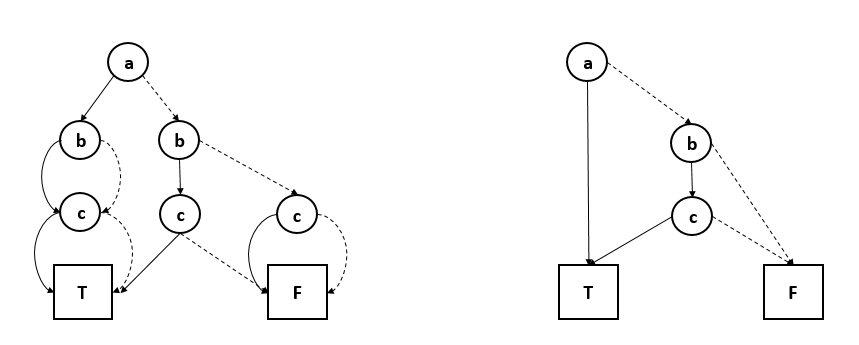
\includegraphics[width=0.8\textwidth] {images/bdd.png}}
        \caption{\label{fig:bdd} Binary Decision Diagrams of the Formula $a \lor (b \land c)$}
\end{figure}
As shown in Figure~\ref{fig:bdd}, it is a rooted, directed, acyclic graph with internal decision nodes and two terminal nodes (\textit{true} and \textit{false}). Each of the decision nodes is labeled with a Boolean variable and has two child nodes, low child and high child. The edge from a node to its low child represents the assignment of \textit{false}, likewise the edge to the high child represents the assignment of \textit{true}. The BDD is called \textit{ordered} if different variables appear in the same order on all paths from the root. Intuitively, following a path from the root to the \textit{true} terminal node represents a valid assignment to the Boolean formula (invalid in the case of ending on the \textit{false} terminal node). 

BDDs are reduced by the removal of isomorphic subgraphs. The BDD shown on the right of Figure~\ref{fig:bdd} is the reduced form of the BDD on the left.
\end{comment}